\chapter{Progettazione}
La fase di progettazione prevede principalmente la scelta dell'architettura da usare, su cui costruire il sistema. 
\\Dato il contesto di utilizzo dell'applicativo, la necessità principale è la sincronizzazione del lavoro dei dipendenti. L'obiettivo è quello di informare ogni dipendente del avvenimento di eventi a cui esso è interessato. Ogni azione deve essere memorizzata nel sistema, in conseguenza della quale esso provvede ad avvisare il gruppo di dipendenti relativo.
\\Ad esempio, al momento della registrazione di un'ordinazione da parte di un cameriere, il sistema provvede a notificare lo chef/pizzaiolo (realizzatore in generale) per informalo della nuova pietanza da preparare.
\\Per identificare l'architettura ideale bisogna elencare quali sono i componenti che ne fanno parte e in che modo sono interconnessi.
\begin{itemize}
	\item I componenti sono di due tipologie:
		\begin{itemize}
			\item Dispositivi utente, rappresentano i dispositivi fisici concessi ai dipendenti (smartphone o applicazione desktop)
			\item Sistema centrale, racchiude la logica di gestione e a cui i dispositivi utente possono fare accesso.
		\end{itemize}
	\item I connettori sono principalmente protocolli di rete, in quanto il sistema è pensato anche per dipendenti che hanno la possibilità di spostarsi all'interno del locale e accedere al sistema centrale in modalità remota.
\end{itemize}
Alla base di ciò i componenti devono ricevere dei cambiamenti del sistema tramite opportune \textit{notifiche}, evitando quindi attese attive.

\section{Architettura}
Sulla base delle necessità descritte in precedenza, si è scelto di utilizzare uno stile architetturale del tipo \textbf{Publish-Subscribe}. Per la realizzazione dell'applicativo infatti vengono ripresi tutti i vantaggi dello stile a \textit{invocazione implicita}:
\begin{itemize}
	\item \textit{Disaccoppiamento spaziale}: tutti i componenti sono altamente disaccoppiati, favorendo la scalabilità del sistema. Il proprietario può quindi assumere un numero di dipendenti variabile senza conseguenze.
	\item \textit{Disaccoppiamento di sincronizzazione}: tutti i componenti non lavorano in "polling", ovvero in attese attive che possono bloccare il sistema.
	\item \textit{Disaccoppiamento temporale}: tutti i componenti possono essere volatili nel sistema.
\end{itemize}
In relazione ai componenti descritti, tutti i dipendenti sono dei \textit{Subscribers} mentre il sistema centrale è l'unico \textit{Publisher}.
\\I dipendenti, effettuando l'accesso, si iscrivono in automatico al Publisher.
Dato che il sistema può contenere un numero notevole di dipendenti, il Publisher fa uso di \textbf{Proxy} per smistare i messaggi solamente a specifici Subscribers.
\\Essi infatti all'atto del login non conoscono i Proxy del sistema, ma è il sistema stesso che li racchiude in gruppi (con lo stesso ruolo) e li associa a determinati Proxy. Tutto ciò si traduce in una distribuzione più efficiente del calcolo computazionale.
\\Riassumendo quindi:
\begin{table}[H]
	\centering
	\begin{tabular}{|l | p{0.75\linewidth} |}
		\hline
		\textbf{Componenti} & Publisher, Subscribers, 
		Proxy \\
		\hline
		\textbf{Connettori} & Protocolli di rete \\
		\hline
		\textbf{Dati} & Notifiche, Richieste di informazioni, Informazioni pubblicate \\
		\hline
		\textbf{Topologia} & Subscribers sono connessi al Publisher indirettamente, ricevendo e inviando notifiche attraverso i Proxy \\
		\hline
		\textbf{Vantaggi} & Subscribers sono tutti disaccoppiati lavorando in parallelo. Le notifiche vengono ben distribuite grazie ai Proxy \\
		\hline
		\textbf{Svantaggi} & Il controllo computazionale è caricato tutto sul sistema centrale. Nessuna conoscenza di quali componenti risponderanno ad un eventi \\
		\hline
	\end{tabular}
\end{table}

\subsection{Main System}
Il sistema principale è l'unico Publisher dello stile utilizzato. Studiando i vari stili architetturali, tra quelli visti durante il corso, e prendendo spunto dallo stile a livelli, l'architettura del sistema non si rispecchia in uno stile architetturale ben preciso, ma è caratterizzata nel seguente modo:
\begin{figure}[H]
	\centering
	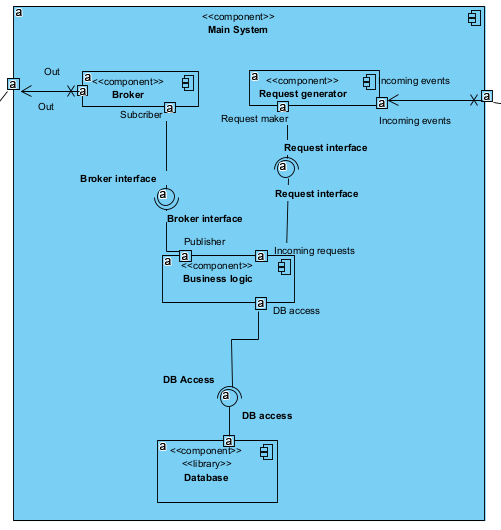
\includegraphics[width=0.4\textwidth]{Immagini/main_system.png}
\end{figure}
\begin{itemize}
	\item \textbf{Database}: Al livello più basso, il componente, racchiude tutte le funzionalità per accedere e modificare i dati all'interno della base di dati del sistema. La business logic accede al database solo attraverso all'interfaccia che tale livello offre, mascherando la reale implementazione.
	\item \textbf{Business Logic}: Al livello centrale, il componente, racchiude tutte le funzionalità per manipolare le richieste e i dati del sistema. Effettua tutti i controlli necessari prima di inviare una risposta. Si occupa principalmente di implementare i casi d'uso.
	\item \textbf{Broker}: Al livello più alto il Broker si occupa solo di inviare i le risposte (prodotte dalla Business Logic) ai diretti interessati. 
	\item \textbf{Request Generator}: Al livello più alto esso riceve, e identifica, le richieste dall'esterno e le inoltra alla Business Logic che si occupa di elaborarle e inviare le risposte al Broker.
\end{itemize}
La Business Logic deve esporre un'interfaccia al Request Generator che contiene le funzioni in relazione al caso d'uso da realizzare.
\\Tutto il componente viene visto dall'esterno (e quindi dai Proxy) come una blackbox con due sole interfacce: una per ricevere delle richieste e una per pubblicare gli eventi.

\subsection{Proxy}
Il proxy contiene un'insieme di utenti connessi al sistema tramite applicazione. Esistono più proxy, ognuno associato ad una categoria di utenti (i.e. Proxy Camerieri è associato a tutti i camerieri). Così facendo, all'atto dell'invio di un messaggio il Broker lo invia ad un relativo Proxy che provvede a smistarlo correttamente. 
\begin{figure}[H]
	\centering
	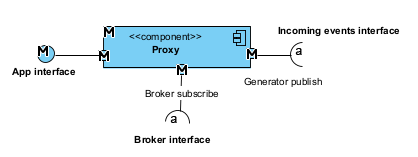
\includegraphics[width=0.6\textwidth]{Immagini/proxy.png}
\end{figure}
Oltre a inviare i messaggi a tutti i dispositivi associati, esso riceve anche informazioni solo da essi.
\\Esso è quindi dotato di tre interfacce:
\begin{itemize}
	\item Un'interfaccia per collegarsi al Broker. Il Broker invia un evento da pubblicare, il proxy lo pubblica a tutti i suoi dispositivi.
	\item Un'interfaccia per collegarsi al Request Generator. Il proxy riceve dai dispositivi eventi di richiesta, il Request Generator riceve da esso l'evento da elaborare.
	\item Un'interfaccia per collegarsi all'applicazione mobile.
\end{itemize}
Attraverso l'analisi degli attori precedentemente descritta si hanno sei tipi di proxy:
\begin{itemize}
	\item Proxy Cameriere associato a tutti i camerieri in servizio.
	\item Proxy Realizzatori associato a tutti i realizzatori di ordinazioni (chef, pizzaiolo, barista).
	\item Proxy Accoglienza associato all'addetto all'accoglienza.
	\item Proxy Cossiere associato al cassiere in servizio.
	\item Proxy Gestione associato al proprietario e all'economo.
	\item Proxy Login è un proxy generale a cui vengono associati tutti gli utenti che non hanno ancora effettuato l'accesso.
\end{itemize}
L'idea di base è che ogni utente, prima di effettuare l'accesso, può contattare solo il \textit{Proxy Login}, il quale provvede in base alle credenziali ad associare il dispositivo al relativo Proxy.

\subsection{Applicazione Mobile}
Tutto il calcolo computazionale è a carico del \textit{Main System}, mentre lo smistamento dei messaggi è a carico dei \textit{Proxy}. L'applicazione deve solo ricevere e inviare eventi al proxy (o ai proxy, se più di uno) associato. La costruzione del messaggio avviene tramite un'interfaccia grafica per ogni contesto, il resto è gestito tutto dal Main System.
\\A tal proposito si è utilizzato il pattern Architetturale \textit{MVC (Model View Control)} per la realizzazione dell'applicazione.
\begin{itemize}
	\item \textit{Modello} contiene tutti i dati necessari per il messaggio da inviare o ricevuto dall'esterno. Nella pratica il modello è una copia del package \textit{Areas} del Main System. I dati infatti vengono scambiati tramite appositi messaggi utilizzato una serializzazione JSON.
	\item \textit{Controllo} contiene tutte le funzionalità per interfacciarsi all'esterno tramite opportuni protocolli di rete per inviare e ricevere messaggi.
	\item \textit{View} è la rappresentazione grafica dei dati.
\end{itemize}

\section{Component Diagram}
\begin{figure}[H]
	\centering
	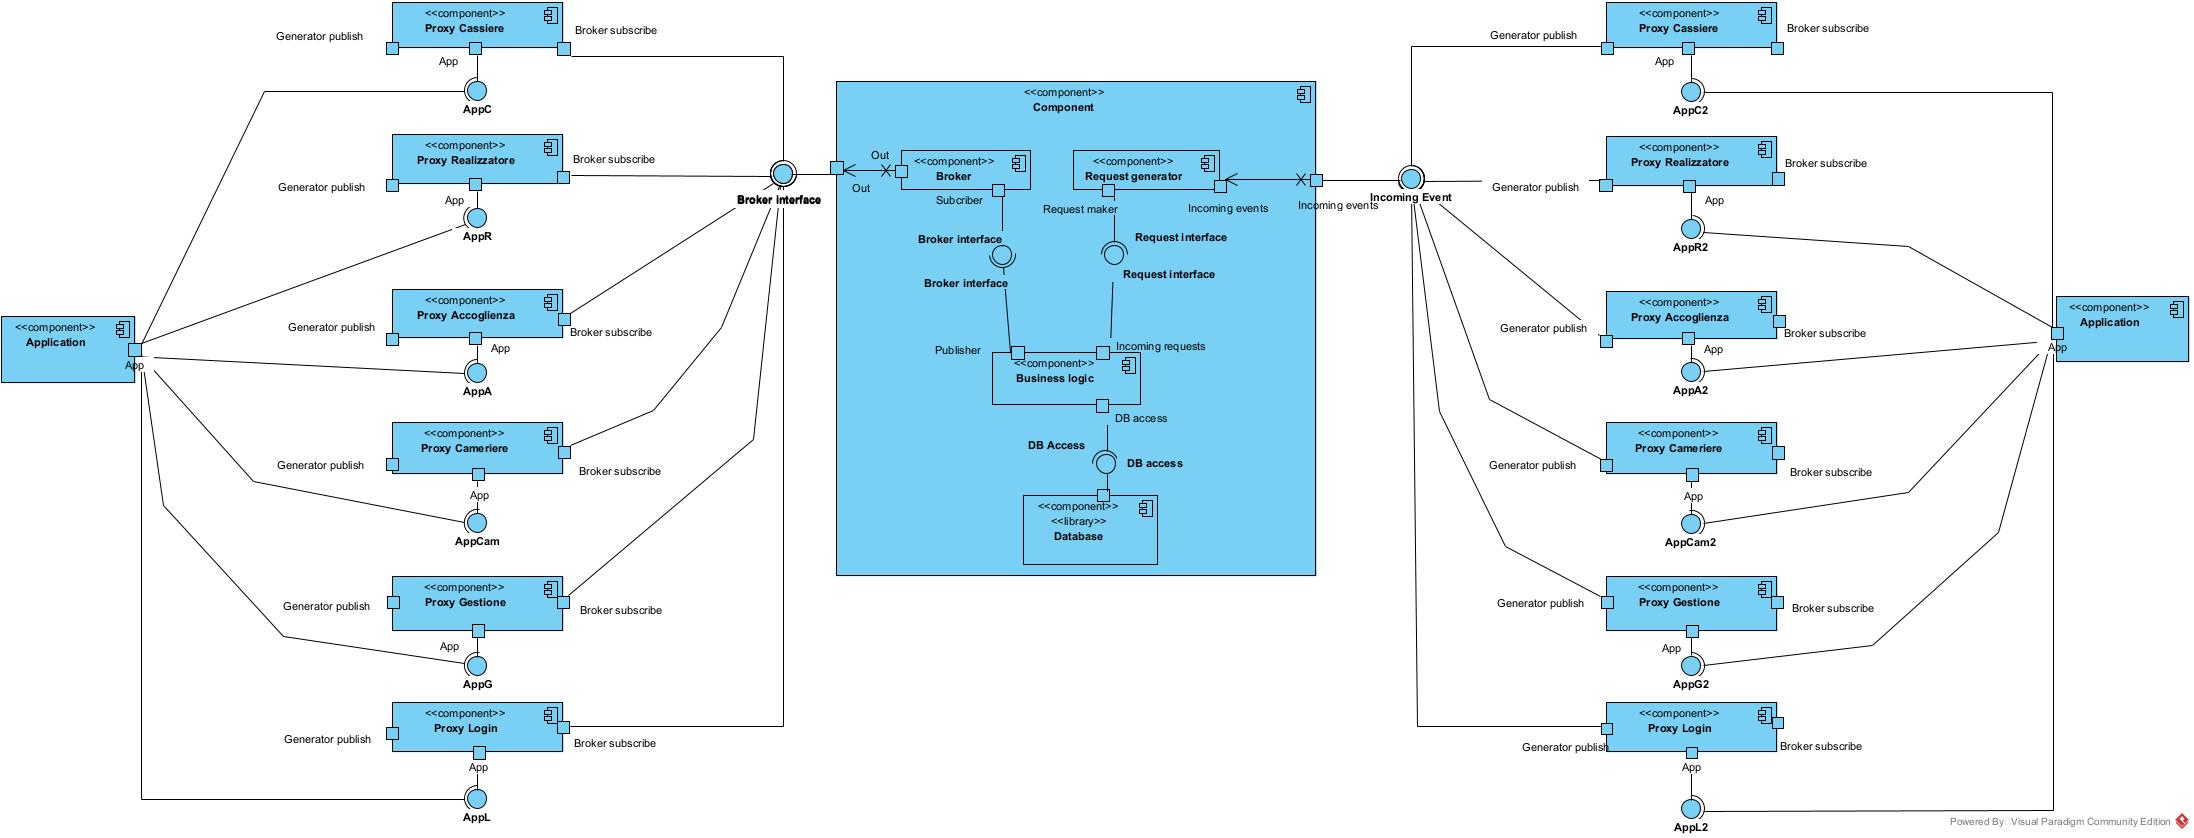
\includegraphics[width=1\textwidth]{Immagini/components.jpg}
\end{figure}
Per rendere più chiara la lettura del diagramma, i proxy sono stati \underline{replicati} solo ad uno scopo grafico. 
\\L'applicazione inoltre non è collegata realmente a tutti i proxy ma solo a quelli a cui corrispondono le sue credenziali di accesso; potenzialmente può essere collegata a tutti i proxy.

\section{Class Diagram}
Dopo aver illustrato il component diagram, si deve illustrare il modello ad oggetti di ogni componente presente nel sistema.


\subsection{Main System}
Il Main System è il componente più complesso perché contiene a sua volta altri componenti connessi tra loro, quindi non può essere rappresentato con un unico class diagram. 
\\Nel livello inferiore è presente il database. Esso non può essere rappresentato come class diagram per la sua natura, inoltre non deve essere realizzato poiché ci si affida a database \textit{relazionali} già esistenti.

\subsubsection{Business Logic}
Il class diagram è diviso in layer orizzontali, in cui ogni livello può interfacciarsi solo con il livello inferiore e può offrire un'interfaccia al livello superiore:
\begin{itemize}
	\item \textbf{DataAccess}: livello più basso si occupa di implementare il driver per l'accesso al database.
	\item \textbf{Areas}: livello centrale mantiene il modello ad oggetti del sistema vero e proprio. Le aree interne comunicano tra loro solo attraverso i loro controllori, richiedendo e fornendo servizi.
	Un esempio è che, pur essendo la TableAndOrdersArea l’area responsabile di generare un ordine, sarà la MenuAndWareHouseArea (gestore del menù) responsabile di inizializzare il prodotto ordinato (dal prodotto del menu) e di ritornarlo all’ordine.
	\\Un altro esempio riguarda sempre la registrazione di un ordine presso un utente.
	\item \textbf{Controller}: livello più alto può accedere al modello inferiore e fornire un'interfaccia per un accesso controllato ai dati.
\end{itemize}
\begin{figure}[H]
	\centering
	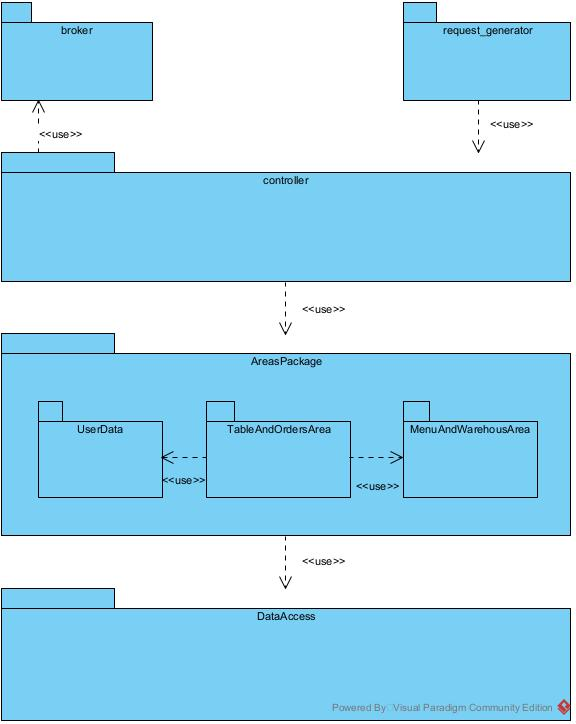
\includegraphics[width=0.6\textwidth]{Immagini/business_logic.jpg}
\end{figure}
\hrule
\vspace{0.5cm}
\textbf{Areas}:
Il livello dei dati è a sua volta diviso in layer verticali. La costruzione di un’area segue sempre lo stesso schema:
\begin{enumerate}
	\item Gli elementi di dominio che offrono operazioni per modificarne lo stato o per ottenere informazioni.
	\item Un controller che permette l’accesso ai servizi del package ma consente anche agli elementi di dominio di richiedere servizi agli altri layer verticali.
\end{enumerate}
Ogni livello si occupa di gestire specifiche macro-responsabilità:
\begin{itemize}
	\item \textit{MenuAndWareHouseArea} si occupa di gestire le richieste di visualizzazione di prodotti sul menu, di merci, di aggiornamento della disponibilità dei prodotti in relazione alle merci ed alla creazione e personalizzazione di prodotti ordinati.
	\item \textit{TableAndOrdersArea} si occupa di gestire lo stato dei tavoli, la creazione degli ordini ad un tavolo e la modifica degli ordini.
	\item \textit{UserData} si occupa di verificare quali siano i ruoli di un utente fornendoli al richiedente, e di registrare gli ordini associati agli utenti.
\end{itemize}
Nel dettaglio i tre package sono progettati nel seguente modo.
\vspace{0.5cm}
\\\textit{MenuAndWareHouseArea}:
\begin{figure}[H]
	\centering
	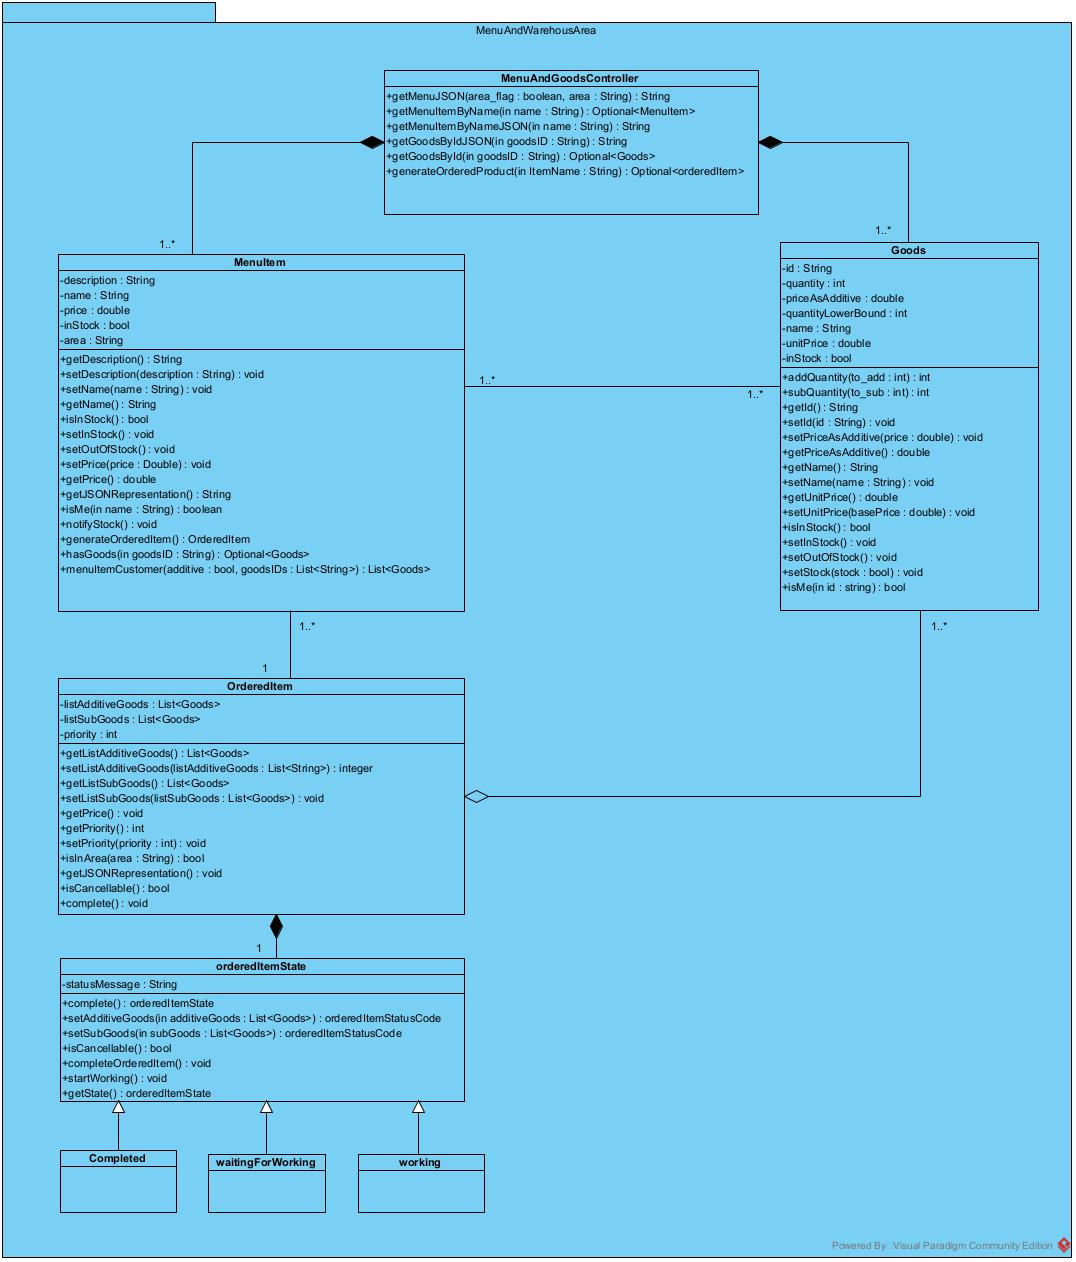
\includegraphics[width=0.8\textwidth]{Immagini/MenuAndWareHouseArea.jpg}
\end{figure}
La classe \textit{orderedItem} in linea con lo state chart descritto nei capitoli precedenti è stato progettato utilizzando il \underline{design patter State} ed è associato a i prodotti del menu.
\vspace{0.5cm}
\\\textit{TableAndOrdersArea}:
\begin{figure}[H]
	\centering
	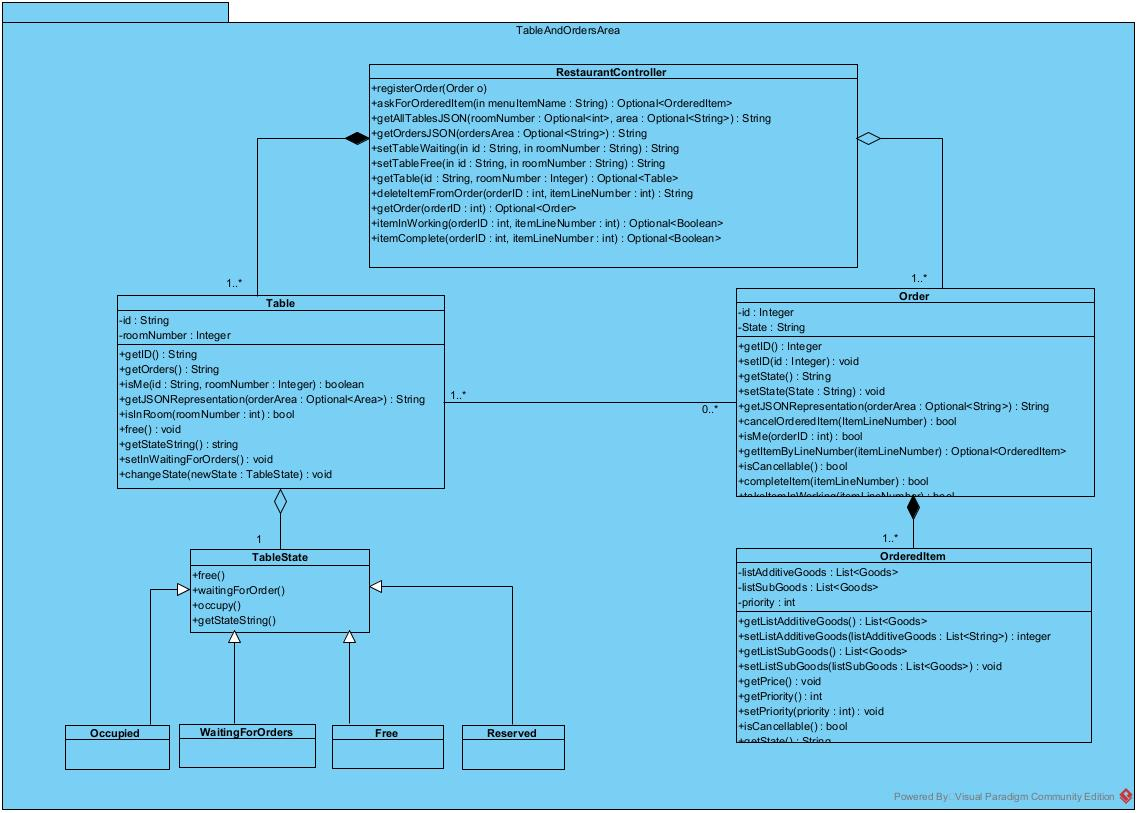
\includegraphics[width=0.8\textwidth]{Immagini/TableAndOrdersArea.jpg}
\end{figure}
Anche in questo caso in linea con lo state chart il \textit{Table} è stato progettato utilizzando il \underline{design patter State}.
\vspace{0.5cm}
\\\textit{UserData}:
\begin{figure}[H]
	\centering
	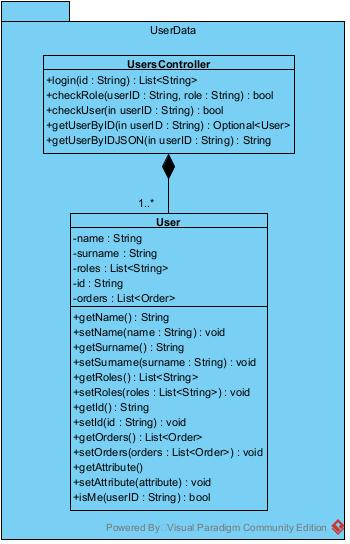
\includegraphics[width=0.3\textwidth]{Immagini/UserData.jpg}
\end{figure}
\vspace{0.5cm}
\hrule
\vspace{0.5cm}
\textbf{DataAccess}:
\begin{figure}[H]
	\centering
	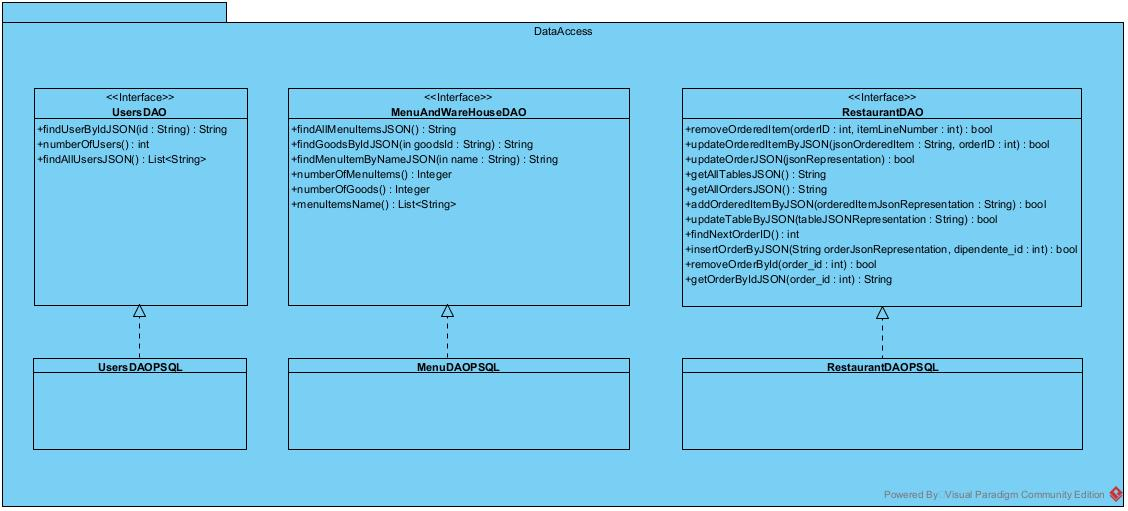
\includegraphics[width=0.8\textwidth]{Immagini/DataAccess.jpg}
\end{figure}
Ad ogni layer verticale del livello superiore è associato una sola classe di accesso del livello inferiore. Così facendo ogni area può accedere solo alla parte di database interessata. 
\vspace{0.5cm}
\hrule
\vspace{0.5cm}
\textbf{Controller}:
\begin{figure}[H]
	\centering
	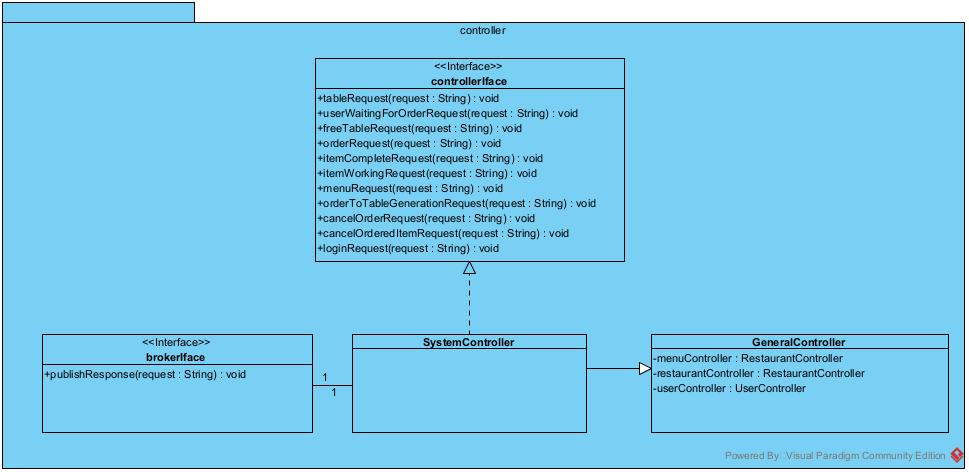
\includegraphics[width=0.8\textwidth]{Immagini/controller.jpg}
\end{figure}
Il \textit{SystemController} offre tutte le funzioni di callback, per prelevare le informazioni necessarie dal modello. Inoltre definisce l’interfaccia che un Broker deve avere qualora voglia ricevere i nuovi eventi generati dalla parte centrale.

\subsubsection{Request Generator}
Si interfaccia con i \textit{Proxy} per ricevere i messaggi e, attraverso un Dispacher, selezionare la funzione di callback del \textit{Controller} giusta per la richiesta. Il Request Generator inoltre definisce l’interfaccia che un Controller deve avere, qualora voglia iscriversi a quest’ultimo come, dualmente, il Controller fa con il Broker.
\begin{figure}[H]
	\centering
	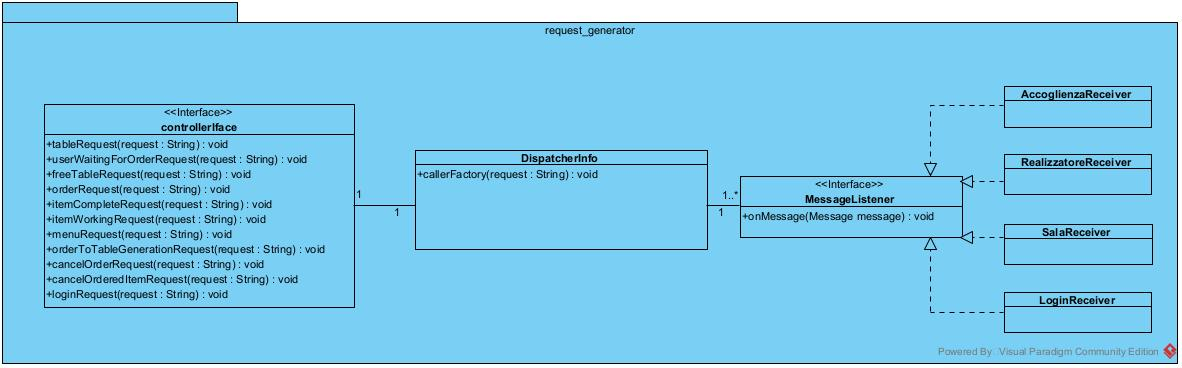
\includegraphics[width=\textwidth]{Immagini/request_generator.jpg}
\end{figure}
La classe \textit{DispatcherInfo} a seconda del messaggio ricevuto chiama una funzione di callback dell'interfaccia di controller.
\\Il \textit{MessageListener} è l'interfaccia di un \textit{Receiver}. Esistono Receiver diversi, poiché i messaggi in arrivo hanno come sorgente Proxy diversi; identicamente però richiamano un'unica funzione del \textit{Dispatcher}.
\\Una seconda soluzione poteva essere di gestire un unico \textit{Receiver} aumentando però la complessità di implementazione. 	

\subsubsection{Broker}
Si interfaccia con i \textit{Proxy} per inviare i messaggi. Il broker come il duale del request generator.
\begin{figure}[H]
	\centering
	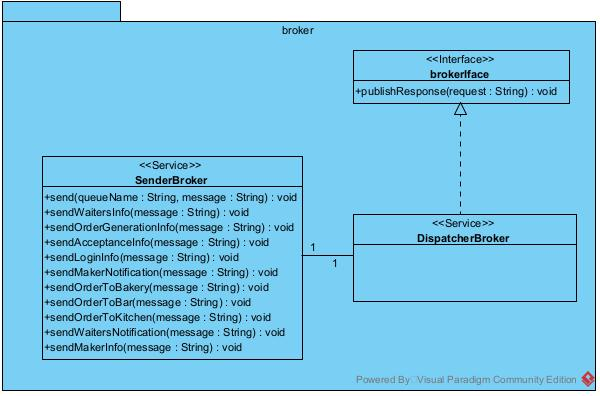
\includegraphics[width=0.6\textwidth]{Immagini/broker.jpg}
\end{figure}
Implementa l'interfaccia con i metodi di callback richiesti dal \textit{SystemController}, a seconda della richiesta viene richiamata uno specifico metodo del \textit{Sender}.
I metodi del \textit{Sender} possono essere di due tipi:
\begin{itemize}
	\item Info: inviano un evento(richiesta) solo a coloro che hanno generato l'evento scatenante.
	\item Notification: inoltrano una notifica. Una notifica è un evento generato dalla Business Logic per informare tutti i Subcribers della verifica di un evento.
\end{itemize}

\subsection{Proxy}
 \begin{figure}[H]
	\centering
	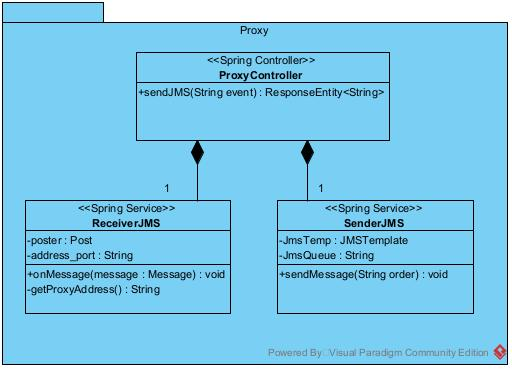
\includegraphics[width=0.5\textwidth]{Immagini/proxy_classdiagram.jpg}
\end{figure}
Lo scopo del Proxy è quello di inviare/ricevere i messaggi a specifici gruppi di utenti. Si occupa quindi di interfacciarsi dualmente con il Main System (attraver il ReceiverJMS e SenderJMS), e di interfacciarsi con le applicazioni esterne.


\subsection{Applicazione Mobile}
In accordo con il pattern MVC quindi, ad alto livello:
\begin{figure}[H]
	\centering
	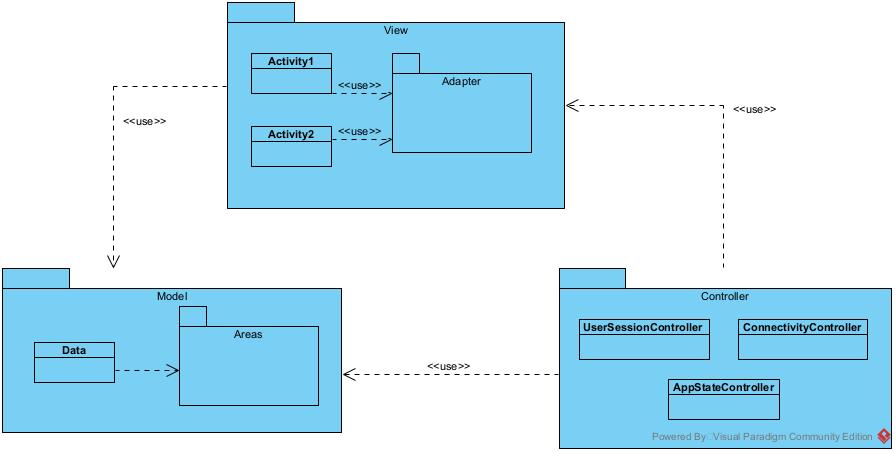
\includegraphics[width=0.8\textwidth]{Immagini/android_classdiagram.jpg}
\end{figure}
Brevemente:
\begin{itemize}
	\item Controller si occupa di gestire gli eventi da e per l'esterno, interagendo con l'utente che utilizza l'applicazione.
	\begin{itemize}
		\item \textit{AppStateController} è una classe realizzata con design pattern \underline{Singleton}. Essa mantiene le informazioni riguardo allo stato dell'applicazione corrente (ad esempio l'activity in esecuzione).
		\item \textit{UserSessionController} mantiene le informazioni riguardo all'utente connesso. Il suo scopo è di identificare il ruolo dell'utente in un particolare contesto e associare il relativo indirizzo del proxy da contattare. Ad esempio se l'utente sceglie di aggiornare lo stato di un tavolo allora è sicuramente con il ruolo di \textit{Addetto all'accoglienza}.
		\item \textit{ConnectivityController} è una classe realizzata con design pattern \underline{Singleton}. Esso mantiene l'unico server in esecuzione che accoglie i messaggi esterni e interagisce con gli altri controller.
	\end{itemize}
	\item Model si occupa di gestire tutti i dati utili all'applicazione. Il package Areas al suo interno è idealmente identico all'omonimo package nella \textit{Business Logic}. In realtà però contiene solo classi e attributi che interessano ai fini dell'utilizzo.
	\\La classe \textbf{Data} è una classe con design pattern \underline{Singleton} poiché all'interno del sistema deve esistere una sola istanza per gestire il modello.
	\item View si occupa di realizzare un'interfaccia grafica dei dati del modello.
\end{itemize}

\section{Database}
Il database deve contenere le informazioni di base che devono essere utilizzate, a partire dai dipendenti che vengono registrati nel sistema e finire con le ordinazioni che vengono effettuate durante l'utilizzo del sistema.
\begin{figure}[H]
	\centering
	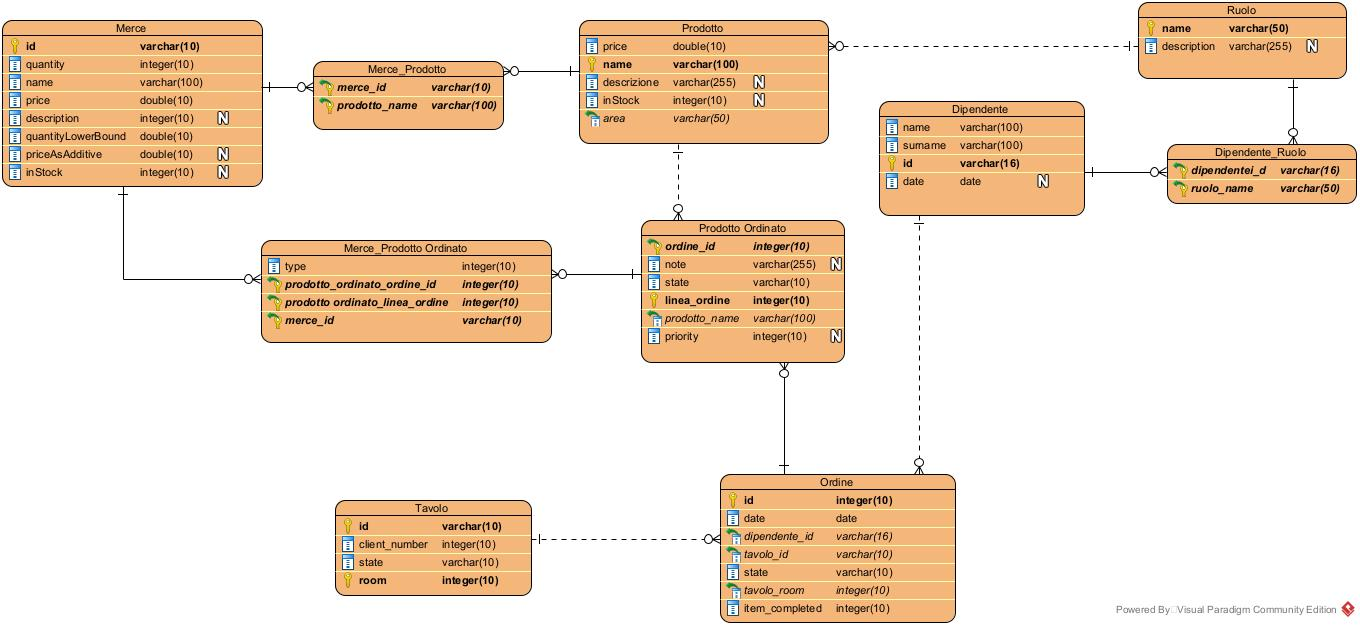
\includegraphics[width=1\textwidth]{Immagini/database.jpg}
\end{figure}
Le caratteristiche principali del database sono le seguenti:
\begin{enumerate}
	\item Le merci hanno, oltre alle informazioni di base quali prezzo, codice identificativo, nome, etc, hanno un attributo \textit{priceAsAdditive}. Tale attributo, se non nullo, indica il prezzo da aggiungere se quella merce è usata come merce aggiuntiva di un prodotto.
	\item Il \textit{Prodotto Ordinato} è un'associazione ternaria tra \textit{Ordine}, \textit{Prodotto} e \textit{Merce}.
	 \item Ogni prodotto ha un attributo collegato all'entità \textit{Ruoli}. Esso serve per indicare a che attività appartiene quel prodotto.
\end{enumerate}
Il precedente database si riferisce solo ai casi d'uso che si sono scelti di implementare. Non contiene, ad esempio, la gestione delle vendite e lo storico del locale.

\section{Sequence Diagram}
I Sequence Diagrams inerenti il Main System sono stati organizzati secondo diversi livelli di dettaglio con una logica a “decomposizione”.
\\Per una apposita lettura ovviamente i Sequence di uno specifico livello di dettaglio iniziano con un determinato prefisso.
\begin{enumerate}
	\item I Sequence top rappresentano il funzionamento dell’intera applicazione, dall’arrivo di un messaggio al Request Generator fino all’arrivo della richiesta al Broker.
	//I sequence top richiamano operazioni offerte dai Controller delle tre aree verticali.
	\\Il loro prefisso è: \underline{”top”}. 
	\item \underline{controllersSequence} sono i Sequence dei Controller verticali dell’Areas.
	Il loro prefisso è dato dal nome dell’area con la lettera minuscola.
	\item \underline{menuAndWareHouseArea}: Sequence delle operazioni del Controller dell’area menu e merci.
	\item \underline{tablesAndOrdersArea}: Sequence dell’area del Controller dell’area ristorante(tavoli ed ordini).
	\item \underline{userData}: Sequence del controller area utente.
\end{enumerate}
Sono stati infine forniti Sequence inerenti il funzionament dei proxy
\\I sequence digram mostrati successivamente sono diagrammi di dettaglio che non mostrano la realizzazione delle chiamate a funzioni di livello più basso. Per esse si rimanda al progetto in Visual Paradigm.

\subsection{Creazione di un'ordine}
Rappresenta il generico meccanismo di generazione di svolgimento di una operazione con generazione di notifiche. In genere ogni evento ha suoi particolari metodi per andare a generare le notifiche (metodi di utilita' generateNotifications, non riportati per non appesantire inutilmente i diagrammi).
\\In questo caso specifico ovviamente le notifiche non sono altro che le comande.
In relazione alla decomposizione descritta precedentemente, per la creazione di un'ordine il SD \textit{top}:
 \begin{figure}[H]
 	\centering
 	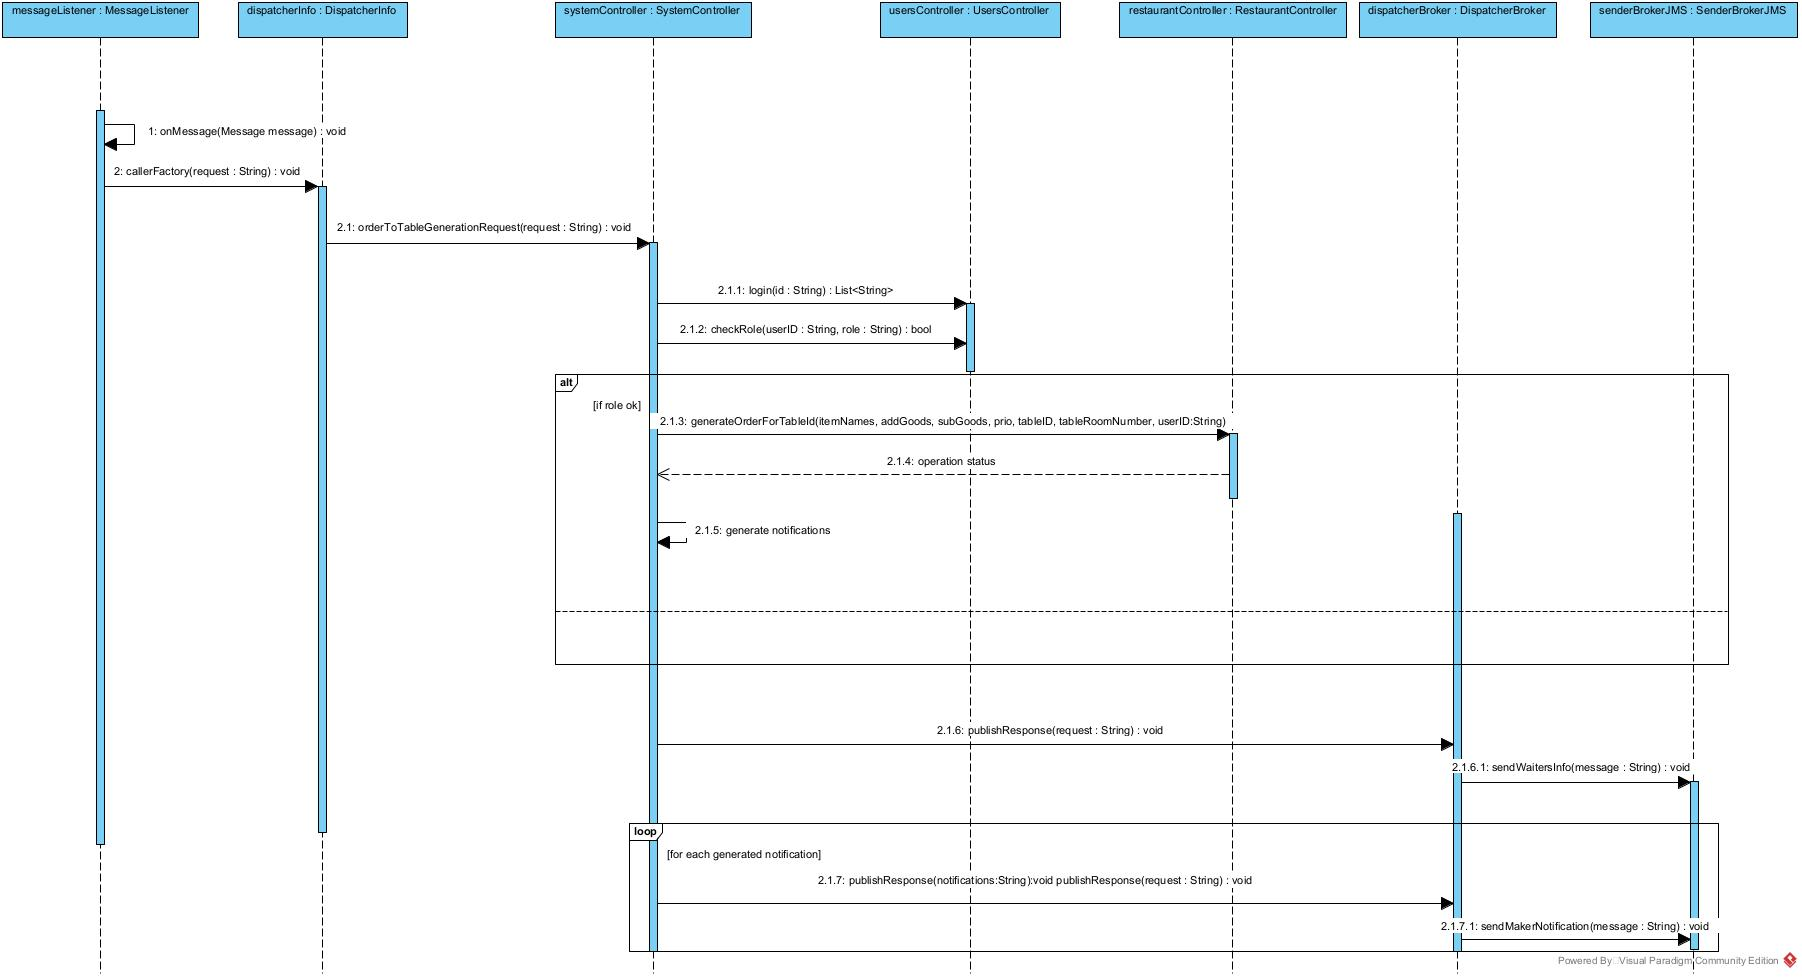
\includegraphics[width=1\textwidth]{Immagini/top_orderToTableGenerationRequest.jpg}
 \end{figure}
Il Sequence precedente utilizza il metodo generateOrderForTableId, il cui SD è il seguente:
 \begin{figure}[H]
	\centering
	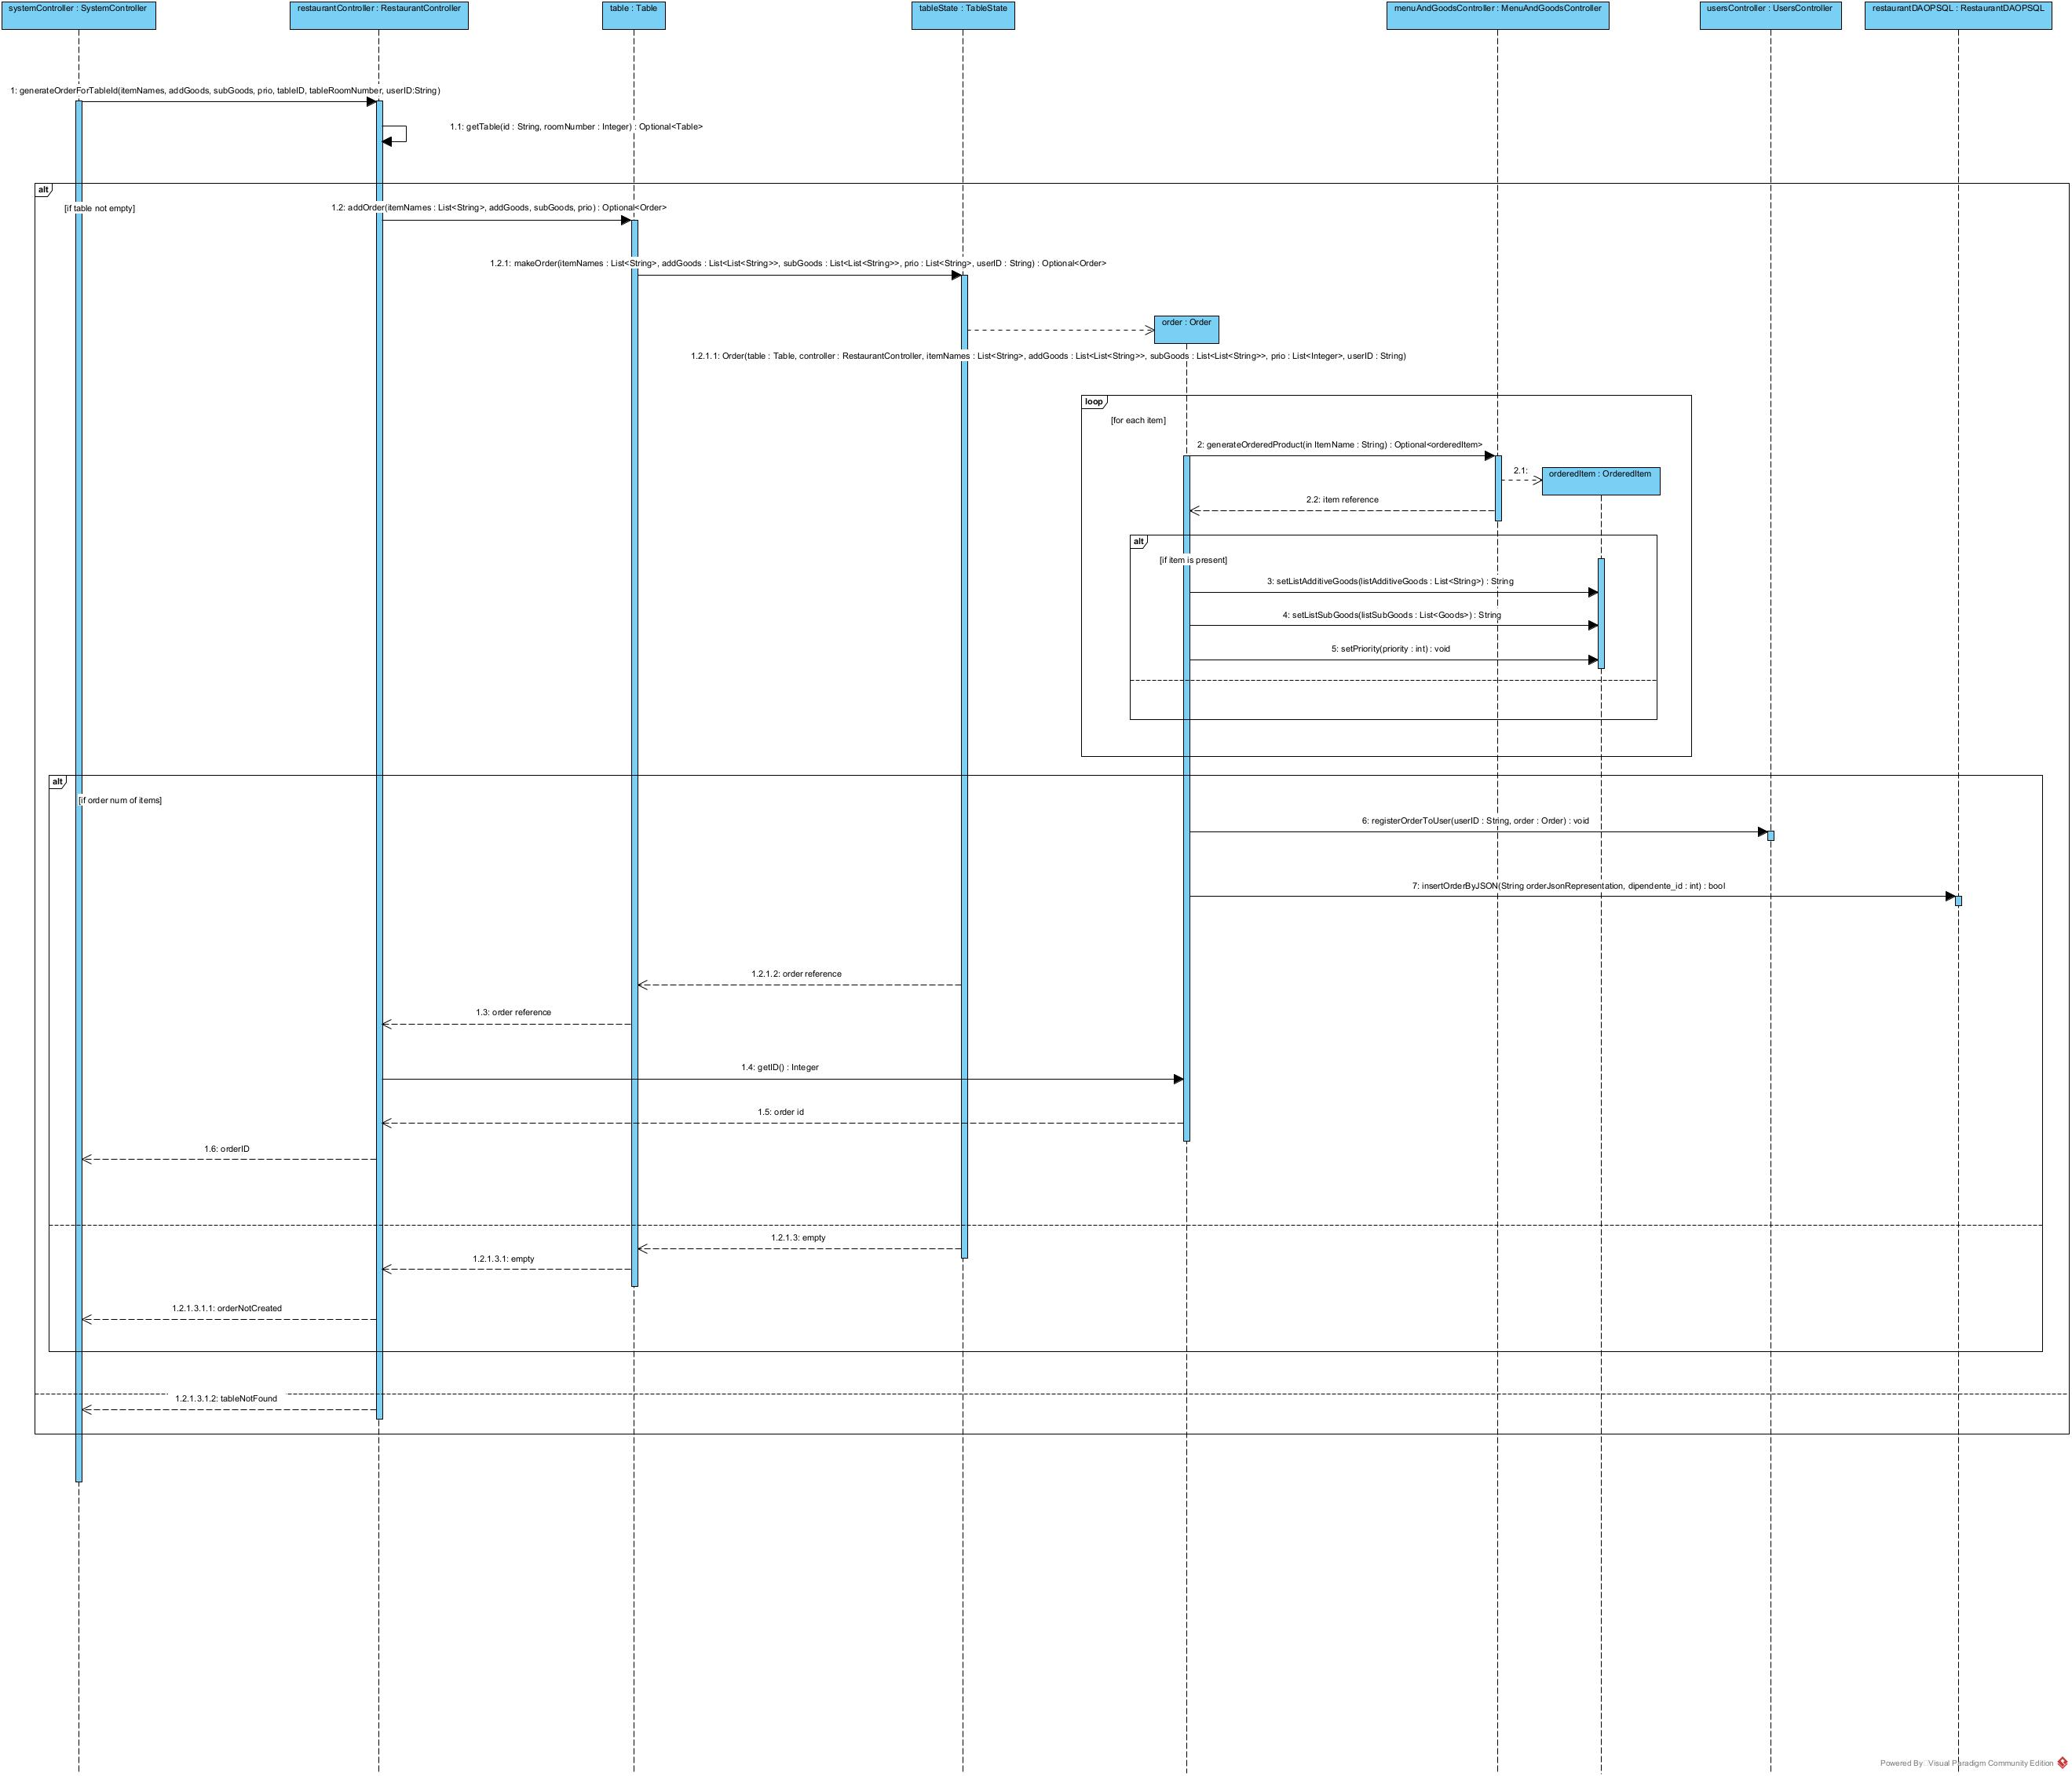
\includegraphics[width=1\textwidth]{Immagini/tableAndOrdersArea_generateOrderForTableId.jpg}
\end{figure}
A sua volta esso richiama il metodo getTable, il cui SSD:
 \begin{figure}[H]
	\centering
	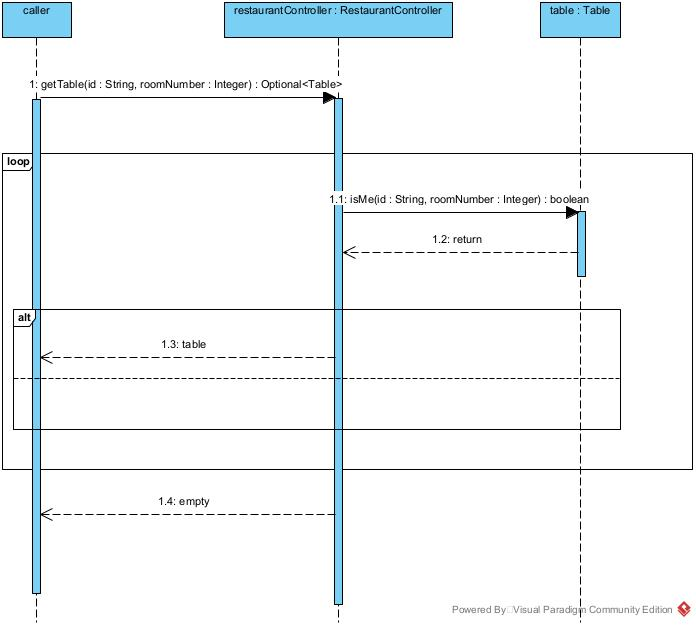
\includegraphics[width=0.6\textwidth]{Immagini/tablesAndOrdersArea_getTable.jpg}
\end{figure}

\vspace{1cm}
Analogamente tutti i SD vengono letti nello stesso modo.

\subsection{Aggiornamento View}
Lato Applicazione Mobile il seguente SD mostra l'interazione nell'MVC per aggiornare la View alla ricezione di un messaggio che contiene un update del modello.
\begin{figure}[H]
	\centering
	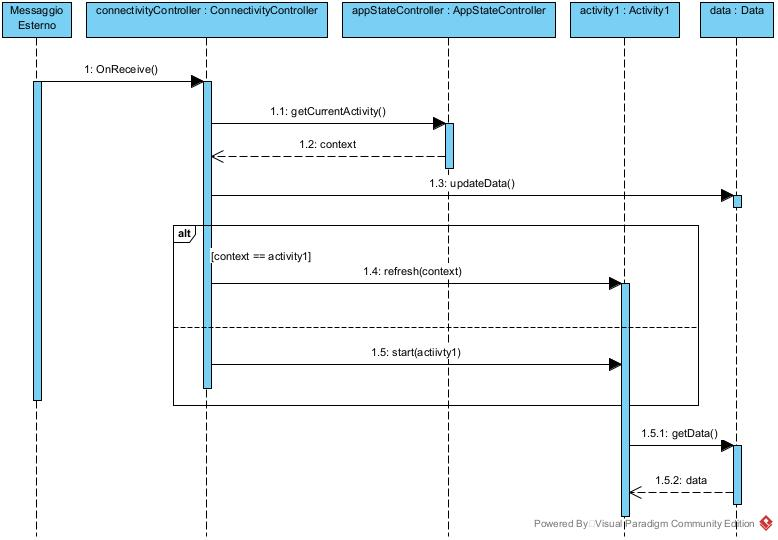
\includegraphics[width=0.8\textwidth]{Immagini/aggiornamento_view.jpg}
\end{figure}
In linea generale il funzionamento è il precedente, ma non è rigidamente rispettato per tutti i possibili casi. Ad esempio in alcuni casi non è necessario richiamare una view, ma solo far visualizzare a video una notifica di aggiornamento.

\section{Deployment Diagram}
\begin{figure}[H]
	\centering
	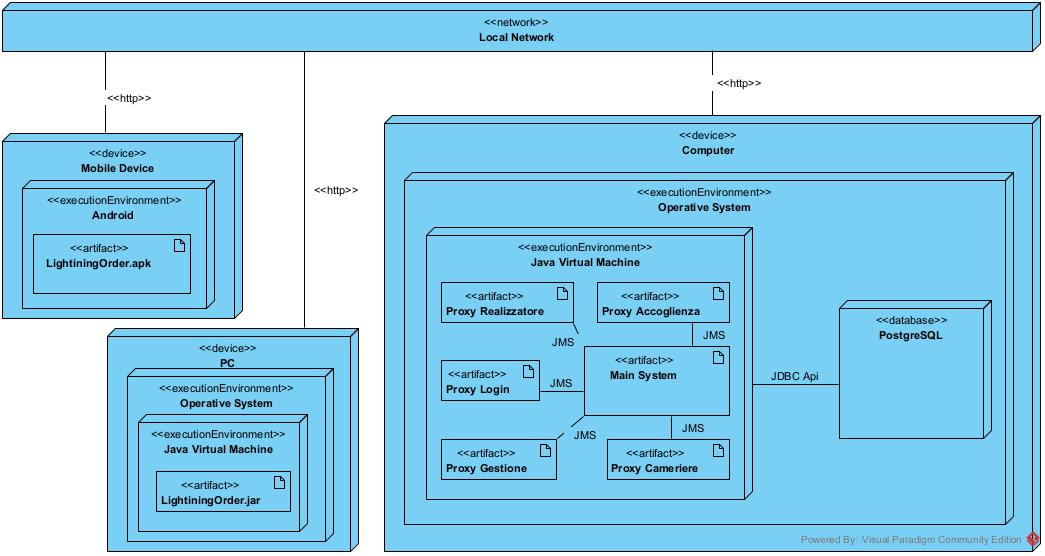
\includegraphics[width=1\textwidth]{Immagini/deploy.jpg}
\end{figure}
I Proxy sono progettati per comunicare tramite JMS quindi non richiedono che siano avviati nella stessa macchina. Essi possono essere collegati anche su altri \textit{device} e poi connessi in rete. Per motivi di mezzi a disposizione si è scelto di avviare i proxy sulla stessa macchina del Main System.
\\Analogo discorso vale per il database.

\section{Messaggi}
Nel sistema vengono scambiati due tipi di eventi:
\begin{itemize}
	\item Richieste.
	\item Notifiche.
\end{itemize}
Le richieste sono eventi che spingono l'applicazione centrale a cambiare stato.
\\Quando un utente si siede ad un tavolo, ad esempio,  l'addetto all'accoglienza genera una richiesta.
L'applicazione centrale, notificata dal Proxy, va a cambiare lo stato del tavolo e produce un "messaggio di risposta".
\\Un messaggio di risposta ad una richiesta arriva sempre mediante chiamata indiretta e riassume il cambiamento dello stato dell'applciazione centrale a seguito dell'evento richiesta.
Nell'esempio precedente all'addetto all'accoglienza, dopo aver generato un evento, sempre in maniera indiretta gli arriva un report che riporta il nuovo stato del tavolo (sempre in maniera indiretta tramite \textit{Webhook}).
Per comodità dunque si indicano come richieste sia gli eventi generati dall'applicazione esterna sia i "messaggi di risposta" alle richieste .
Nonostante i nomi, come già accennato, questi funzionano mediante un meccanismo di invocazione indiretta, sono di fatto delle vere e proprie \textbf{notifiche} (Al sistema centrale viene notificato che un cliente si e' seduto ed all'addetto viene notificata l'avvenuto cambio di stato).
\\Si riconsideri ora l'esempio:
Una volta che il cliente si è seduto e che lo stato è cambiato, è necessario notificare ai camerieri che devono andare a prendersi l'ordinazione. Chi deve pero' generare questa notifica? Secondo lo stile adottato l'applicazione ha originalmente generato un evento gestito solo dall'applicazione centrale che va dunque anche l'onere di notificare i camerieri.
E' dunque compito dell'applicazione centrale andare a generare degli eventi che chiamiamo notifiche.
\\Nell'esempio l'applicazione centrale oltre alla risposta alla richiesta (inoltrato al proxy accoglienza) genera una notifica che, inoltrata al proxy camerieri, viene inviata in broadcast, notificando di fatto i camerieri.
\\Si puo' quindi riassuntivamente dire che:
\begin{itemize}
	\item Richieste: Sono gli eventi generati dagli utenti tramite l'applicazione.
	\item Notifiche: Sono gli eventi generati dall'applicazione centrale in seguito ad una richiesta.
\end{itemize}
Richieste e notifiche vengono inviate tramite appositi messaggi. Un messaggio funge da "stampino" per una richiesta/notifica, ossia gli offre un insieme di campi base. Il significato di quei campi dipende pero' dalla specifica richiesta/notifica.
\begin{figure}[H]
	\centering
	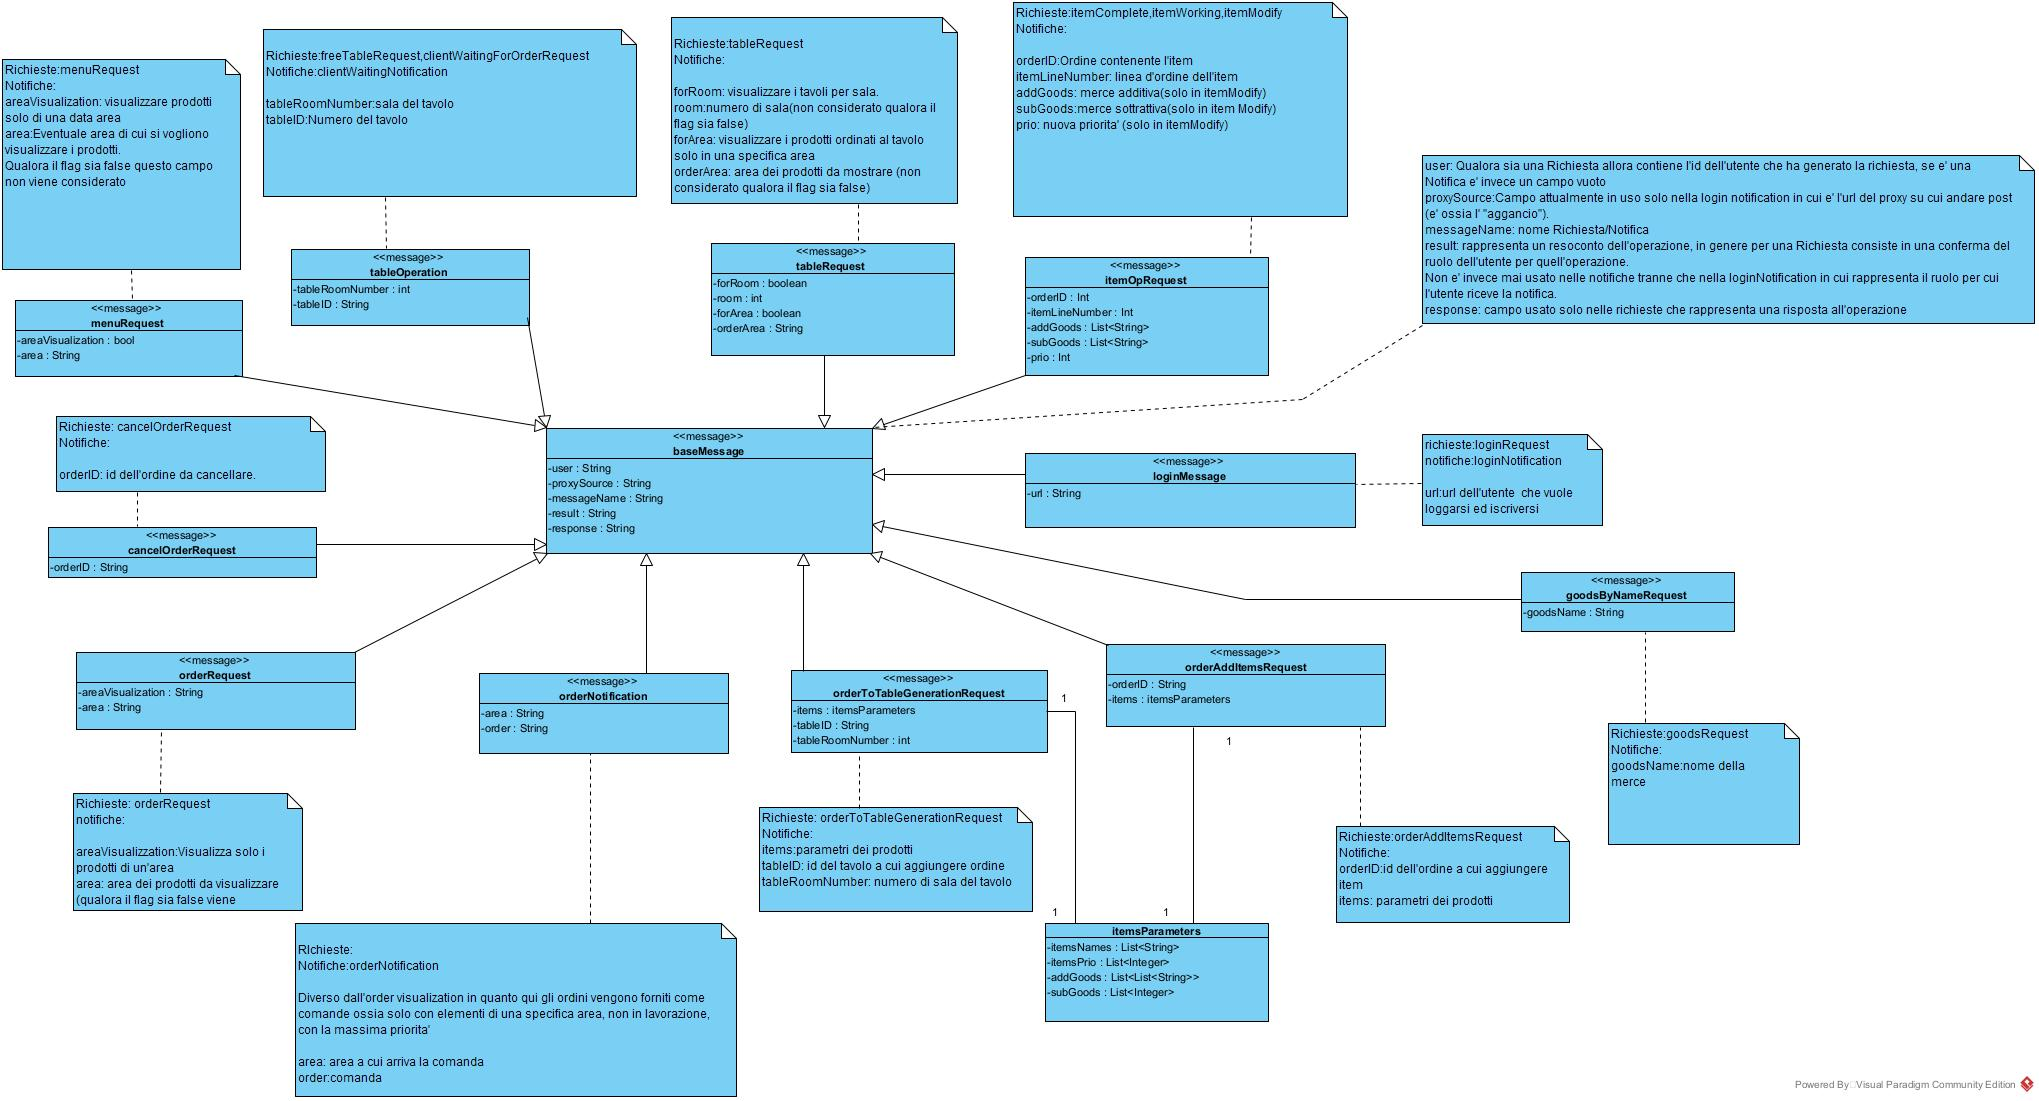
\includegraphics[width=1\textwidth]{Immagini/messages_api.jpg}
\end{figure}

\subsection{Liste di Richieste}
menuRequest: Richiedi una lista di menu
\\freeTableRequest: Un tavolo si e' liberato
\\clientWaitingForOrderRequest: dei clienti sono stati fatti accomodare
\\tableRequest: visualizzare tavoli ed ordini connessi(usata sia da camerieri che da accoglienza)
\\itemComplete: un realizzatore ha terminato un prodotto ordinato(il pizzaiolo ha finito la pizza)
\\itemWorking: un realizzatore ha iniziato a lavorare ad un prodotto
\\itemModify: un cameriere su richiesta del cliente modifica il prodotto
\\cancelOrderRequest: cancellare un ordine
\\orderRequest: un realizzatore vuole visualizzare la lista di ordini presenti nel locale
\\orderToTableGenerationRequest: Un cameriere genera un ordine ad un tavolo
\\orderAddItemsRequest:aggiungi dei prodotti ad un ordine
\\goodsRequest: visualizza della merce per  uno specifico nome
\\loginRequest: un utente desidera loggarsi ricevendo la sua lista di ruoli

\subsection{Lista di Notifiche}
clientWaitingNotification: un cliente e seduto al tavolo attenenendo di compiere la prima ordinazione
\\orderNotification: notifica generata in seguito all'aggiunta di un ordine, al completamento di tutti gli ordini con una data priorita' o all'aggiunta di nuovi ordini. Coincide di fatto con una comanda.
\\loginNotification: notifica che un proxy invia all'utente per notificarlo della sua avveuta sottoscrizione (contiene l'indirizzo del proxy su cui andare po ad effettuare post).

\subsection{Scenario di comunicazione}
Nell'esempio sotto riportato viene rappresentata la comunicazione tra applicazione mobile e Main System attraverso il messaggio \textit{loginRequest}.
\begin{figure}[H]
	\centering
	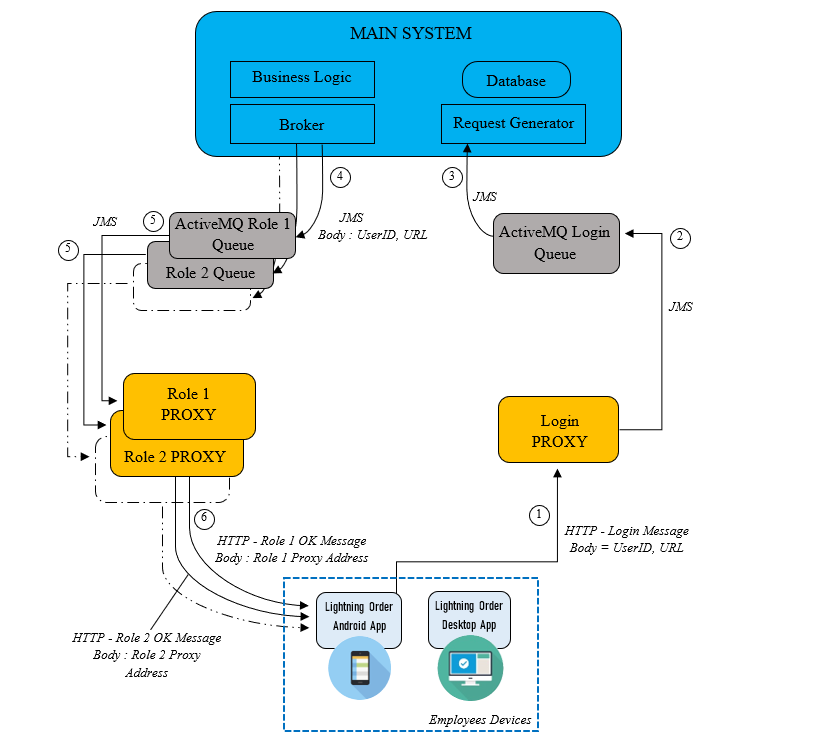
\includegraphics[width=0.7\textwidth]{Immagini/loginScenario.png}
\end{figure}
Il contenuto informativo è rappresentato da stringe di tipo JSON.
